
\chapter{Latency Insertion Method}\label{chap:lim}
    
\section{Rationale for using LIM for Quantized State Simulation}

In order to apply Quantized State System (QSS) integration methods, the study system must be described fully by a set of differential equations without any instantaneous coupling between any of the state variables in the system \cite{cellier2008}. To achieve this, we will use a modeling approach called the Latency Insertion Method (LIM). The LIM, described in \cite{schutt2001} exploits existing latency in the network and inserts small, fictitious latency at nodes and branches where no significant physical latency exists. It provides generic node and branch models, that can be combined into arbitrarily complex typologies to model various electrical devices (or any dynamical devices that can be modeled with an equivalent circuit model). The equivalent circuit model representation is powerful because it imposes conservation law inherently, and it is flexible enough to model dynamical subsystems of many engineering disciplines (mechanical, thermal, etc.). 

With latency at every system node and on every system branch, there is no instantaneous coupling between any states. One way to understand this is to imagine a state space system with no off-diagonal components in the state matrix. All of state coupling occurs within a dynamically-updated input vector. And, although there are proposed versions of the LIM for dealing with algebraic sub-networks \cite{sekine2009}, these methods do not create a model that can be QDEVS compliant. We will therefore focus on creating fully latent networks using the original LIM formulation. 

\section{Atomic LIM Components}

The LIM method uses two primary generic components from which the network model can be developed: a LIM \emph{node} and a LIM \emph{branch}. The LIM node defines a KCL-based ODE for the state of a node voltage, and the LIM branch defines a KVL-based ODE for the current flow between two arbitrary nodes. For the QDL method development, we will use the extended LIM node and branch formulations that include dependent sources as described in \cite{goh2011}. This extended formulation provides a straight-forward means of modeling energy-conversion coupling circuits, which are common in power system models.

\begin{figure}[ht]
    \centering
    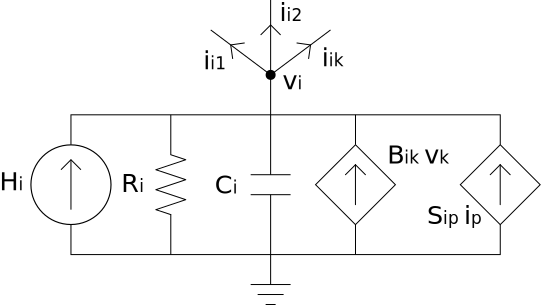
\includegraphics[width=0.7\linewidth]{lim_dependent_node.png}
    \caption{Generic LIM Node with Dependent Sources}
    \label{fig:lim_dependent_node}
\end{figure}

The generic LIM branch model with dependent sources is shown in figure \ref{fig:lim_dependent_node}. The model includes a voltage-controlled current source (VCCS) and a current-controlled current source (CCCS). The KCL equation for the $i^{th}$ node is

\begin{equation} \label{eq:lim_dependent_node}
C_i \frac{d}{dt} v_i(t) + G_i v_i(t) - H_i(t) - B_{ik} v_k(t) - S_{ip} i_p(t) = \sum_{M_i}^{k=1}{i_{ik}(t)}
\end{equation}

Note that these parameters, injections and coefficients can be time-varying and non-linear in general. 

\begin{figure}[ht]
    \label{fig:lim_dependent_branch}
    \centering
    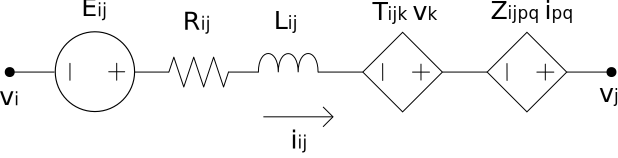
\includegraphics[width=0.8\linewidth]{lim_dependent_branch.png}
    \caption{Generic LIM Branch with Dependent Sources}
\end{figure}

The generic LIM branch model with dependent sources is shown in figure \ref{fig:lim_dependent_branch}. The model includes a voltage-controlled voltage source (VCVS) and a current-controlled voltage source (CCVS). The KVL equation for a branch from $i^{th}$ to the $j^{th}$ node is

\begin{equation} \label{eq:lim_dependent_branch}
v_i(t)-v_j(t) = L_{ij} \frac{d}{dt} i_{ij}(t) + R_{ij} i_{ij}(t) - e_{ij}(t) - T_{ijk}v_k(t) - Z_{ijpq} i_{pq}(t)
\end{equation}

Note that these parameters, injections and coefficients can be time-varying and non-linear in general.  

The LIM formulation also allows for externally-controlled, ideal current source branches and voltage source nodes (see figs. \ref{fig:lim_const_node} and \ref{fig:lim_const_branch}). Although these components are somewhat trivial, they are useful in the derivation of many device models and are worth noting. Because the voltages at the branch ports are effectively dc quantities (as far as the branch model is concerned) during the span of a time step, an ideal source does not require any special consideration by the branch model. Note that ideal voltage nodes may not be added in parallel attached to the same electrical node, and ideal current source branches may not be added in series with other branch models.  

\begin{figure}[ht]
    \label{fig:lim_const_node}
    \centering
    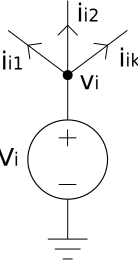
\includegraphics[width=0.18\linewidth]{lim_const_node.png}
    \caption{Ideal Voltage Source Node}
\end{figure}

\begin{figure}[ht]
    \label{fig:lim_const_branch}
    \centering
    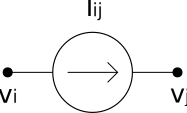
\includegraphics[width=0.24\linewidth]{lim_const_branch.png}
    \caption{Ideal Current Source Branch}
\end{figure}

\section{LIM System Model} 

It is convenient to represent a LIM system model as a state space model, with partitions as shown in (eq. \ref{eq:lim_state_space}). By definition, the LIM state space model does not contain an algebraic output equation but is described fully with the state equation $\dot{\mathbf{x}}(t) = \mathbf{A}\mathbf{x}(t) + \mathbf{B}\mathbf{u}(t)$. The motivation for developing the LIM system state space model is two-fold. We wish to provide a trusted benchmark solution with which to compare QDL simulation accuracy and computational performance, and the state space model is a common format that can be solved with various third-party tools. Also, various components of the LIM state space model will be used directly in the formulation of the QDL atomic model equations described in chapter \ref{chap:qdl}. 

\begin{equation} \label{eq:lim_state_space}
    \frac{d}{dt}
    \begin{bmatrix}
        v \\
        i
    \end{bmatrix}
    = 
    \begin{bmatrix}
        C^{-1}(B-G)   & C^{-1}(S-A) \\
        L^{-1}(T-A^T) & L^{-1}(Z-R)
    \end{bmatrix}
    \begin{bmatrix}
        v \\
        i
    \end{bmatrix}
    +
    \begin{bmatrix}
        C^{-1}  & 0      \\
        0       & L^{-1}
    \end{bmatrix}
    \begin{bmatrix}
        H \\
        E
    \end{bmatrix}
\end{equation}

where: 
\smallskip

$\begin{aligned}
    v & : \text{ the set of node voltages of length } n \\
    i & : \text{ the set of branch currents of length } k \\
    C & : \text{ the set of node shunt capacitance values of length } n \\
    G & : \text{ the set of node shunt conductance values of length } n \\
    H & : \text{ the set of node shunt current injections of length } n \\
    B & : \text{ the set of node VCCS gains of size } (n \times n) \\
    S & : \text{ the set of node CCCS gains of size } (n \times k) \\
    L & : \text{ the set of branch series inductance values of length } k \\
    R & : \text{ the set of branch series resistance values of length } k \\
    E & : \text{ the set of branch series voltage sources of length } k \\
    T & : \text{ the set of branch VCVS gains of size } (k \times n) \\
    Z & : \text{ the set of branch CCVS gains of size } (k \times k) \\
    A & : \text{ the port connection incidence matrix size } (n \times k) \\
\end{aligned}$

\bigskip
and the elements of the incidence matrix $A$ are determined by
\smallskip

\begin{equation} \label{eq:a_matrix}
    A_{i, k} = 
    \begin{cases}
        1,  & \text{if the } i^{th} \text{ node is connected to the } i^{th} \text{ terminal of the } k^{th} \text{ branch }\\ 
        -1, & \text{if the } i^{th} \text{ node is connected to the } j^{th} \text{ terminal of the } k^{th} \text{ branch }\\ 
        0,  & \text{otherwise}
    \end{cases}
\end{equation}

\bigskip

\section{Example LIM System Derivation} 

In order to provide a concrete example of a simple power system formulated using LIM, a dc motor model is presented (fig. \ref{fig:qdl_dc_motor}). This system includes an electro-mechanical energy conversion in the form of back-to-back VCVS and CCCS sources. 

\begin{figure}[ht]
    \label{fig:qdl_dc_motor}
    \centering
    \includegraphics[width=1.0\linewidth]{qdl_dc_motor.png}
    \caption{Example DC Motor System LIM Model with Dependent Sources}
\end{figure}

\bigskip
The LIM system is then defined with the following components:
\bigskip

\begin{equation} \label{eq:lim_sys_1}
v = [v_a \ \ \omega_m \ \ \omega_L]^\intercal,  \ \ \ 
i = [i_a \ \ \tau_s]^\intercal    \\
\end{equation}

\begin{equation} \label{eq:lim_sys_2}
H = [V_g G_g \ \ 0 \ \ T_L]^\intercal,  \ \ \ 
E = [0 \ \ 0]^\intercal    \\
\end{equation}

\begin{multline} \label{eq:lim_sys_3}
R =
\begin{bmatrix}
R_a &  0 \\
0   &  0 \\
\end{bmatrix} ,  \ \ 
L =
\begin{bmatrix}
L_a &  0 \\
0   &  J_p \\
\end{bmatrix} ,  \ \
G =
\begin{bmatrix}
G_g &  0    &  0   \\
0   &  B_m  &  0   \\
0   &  0    &  B_L \\
\end{bmatrix} ,  \ \  \\
C =
\begin{bmatrix}
C_{lim} &  0    &  0   \\
0       &  J_m  &  0   \\
0       &  0    &  J_L \\
\end{bmatrix} ,  \ \
S =
\begin{bmatrix}
0   &  0 \\
K_t &  0 \\
0   &  0 \\
\end{bmatrix} ,  \ \
T =
\begin{bmatrix}
0  &  K_e  &  0  \\
0  &  0    &  0  \\
\end{bmatrix} ,  \ \
A =
\begin{bmatrix}
    1 &  0 \\
    1 &  0 \\
    0 & -1 \\
\end{bmatrix}  
\end{multline}

Note that the armature terminal node does not include any real latency, and so a small, fictitious capacitance of $C_{lim}$ is included in order to ensure that the system has full latency and can be represented by a valid LIM system model. 
